\documentclass[12pt]{article}
\usepackage[a4paper, margin=2.5cm]{geometry} % Set A4 paper size and margins
\usepackage{amsmath} % for mathematical symbols...
\usepackage{amsfonts} % for mathematical fonts
\usepackage[most]{tcolorbox}
\usepackage{tikz}
\usepackage{enumitem}
\usepackage{styles/custome} % custome styles here


\title{Algebra II - Zapiski predavanj}
\date{}
\author{Amar Ustavdić}
\renewcommand{\contentsname}{Vsebina}


\begin{document}

\maketitle
\clearpage 

\tableofcontents
\clearpage

\section{Osnovne algebrske strukture}

\subsection{Algebrska struktura}

\subsubsection{Definicija}
Naj bo $S$ poljubna neprazna množica. \\
Vsaki preslikavi $\varphi : S \times S \to S$ rečemo DVOMESTNA NOTRANJA OPERACIJA \\ (ali DNO) na množici $S$. \\[1em]
Sliko urejenega para $(a, b) \in S \times S$ pišemo $a\varphi b$ (namesto običajnega zapisa $\varphi(a, b)$) \\ in jo imenujemo KOMPOZITUM (SESTAV) ELEMENTOV $a$ in $b$ iz $S$. \\[1em]
Dvomestno notranjo operacijo označujemo z znaki: $+, \cdot, \circ, *,\triangle, \heartsuit, \dots$

\subsubsection{Zgled}
\begin{enumerate}[label=\alph*)]
    \item $S = \mathbb{N}$ \\ $\circ$ je običajno seštevanje naravnih števil. \\ $\Rightarrow$ je DNO, saj $\forall a, b \in \mathbb{N}$ je $a \circ b \in \mathbb{N}$.
    \item $S = \mathbb{N}$ \\ $\circ$ je običajno odštevanje naravnih števil. \\ $\Rightarrow$ ni DNO, npr. za $1 \circ 2 = 1 - 2 = -1 \notin \mathbb{N}$.
\end{enumerate}

\subsubsection{Definicija}
DNO $\circ$ na množici $S \ne \emptyset$ je ASOCIATIVNA če za vse elemente $a, b, c \in S$ velja
\begin{align*}
    (a \circ b) \circ c = a \circ (b \circ c)
\end{align*}
KOMUTATIVNA, če za vsaka elementa $a, b \in S$ velja
\begin{align*}
    a \circ b = b \circ a
\end{align*}

\subsubsection{Zgled}
\begin{enumerate}[label=\alph*)]
    \item $S = \mathbb{Z}$ \\ $\circ$ je običajno seštevanje celih števil. \\ $\Rightarrow$ je DNO. \\ $\Rightarrow \circ$ je komutativna, in je asociativna.
    \item $S = \mathbb{Z}$ \\ $\circ$ je običajno odštevanje celih števil. \\ $\Rightarrow$ je DNO.
    \begin{align*}
        a &= 1, b = 0 \\
        a \circ b &= 1 - 0 = 1 \\
        b \circ a &= 0 - 1 = -1   
    \end{align*}
    $\Rightarrow$ ni komutativna.
    \begin{align*}
        a = 1, b &= 2, c = 3 \\
        (a \circ b) \circ c = & (1 - 2) - 3 = -4 \\
        a \circ (b \circ c) = & 1 - (2 - 3) = 2   
    \end{align*}
    $\Rightarrow$ ni asociativna.
    \item $S = \mathbb{R}^{n \times n}$ (kvadratne matrike z realnimi koeficienti) \\ $\circ$ je običajno množenje matrik. \\ $\Rightarrow$ je DNO, ker je rezultat zmnožka spet kvadratna matrika velikosti $n \times n$ z realnimi koeficienti.
    \begin{align*}
        A = 
        \begin{bmatrix}
            a_1 & b_1 \\
            c_1 & d_1 \\
        \end{bmatrix}, 
        B = &
        \begin{bmatrix}
            a_2 & b_2 \\
            c_2 & d_2 \\
        \end{bmatrix},
        C = 
        \begin{bmatrix}
            a_3 & b_3 \\
            c_3 & d_3 \\
        \end{bmatrix} \\
    \end{align*}
    $\Rightarrow$ je asociativno.
    \begin{align*}
        A = 
        \begin{bmatrix}
            1 & 1 \\
            1 & 1 \\
        \end{bmatrix}, 
        B = 
        \begin{bmatrix}
            1 & 1 \\
            0 & 0 \\
        \end{bmatrix} \\[1em]
        A \circ B = 
        \begin{bmatrix}
            1 & 1 \\
            1 & 1 \\
        \end{bmatrix} \cdot 
        \begin{bmatrix}
            1 & 1 \\
            0 & 0 \\
        \end{bmatrix}
        = 
        \begin{bmatrix}
            1 & 1 \\
            1 & 1 \\
        \end{bmatrix} \\[1em]
        B \circ A = 
        \begin{bmatrix}
            1 & 1 \\
            0 & 0 \\
        \end{bmatrix} \cdot 
        \begin{bmatrix}
            1 & 1 \\
            1 & 1 \\
        \end{bmatrix} =
        \begin{bmatrix}
            2 & 2 \\
            0 & 0 \\
        \end{bmatrix}
    \end{align*}
    $\Rightarrow$ ni komutativno.
\end{enumerate}

\subsubsection{Trditev}
Če je DNO $\circ$ na $S \ne \emptyset$ asociativna, potem je produkt (kompozitum) elementov 
$$a_1, a_2, \dots, a_n \in S \text{ } \text{ } \text{ } (n \in \mathbb{N})$$ 
natančno določen z vrstnim redom teh elementov. Tak produkt označimo z
$$a_1 \circ a_2 \circ \dots \circ a_n$$

\paragraph{Dokaz:}
izpustimo!

\subsubsection{Trditev}
Če je $\circ$ asociativna in komutativna DNO na $S \ne \emptyset$, potem je naš produkt elementov
$$a_1, a_2, \dots, a_n \in S \text{ } \text{ } \text{ } (n \in \mathbb{N})$$
enolično določen ne glede na vrstni red naših elementov.

\paragraph{Dokaz:}
izpustimo!

\subsubsection{Definicija}
Naj bo $S \ne \emptyset$ z DNO $\circ$. \\[1em]
Element $l \in S$ je LEVI NEUTRALNI ELEMENT v množici $S$, če za $\forall a \in S$ velja
$$l \circ a = a$$ \\[1em]
Element $d \in S$ je DESNI NEUTRALNI ELEMENT v množici $S$, če za $\forall a \in S$ velja
$$a \circ d = a$$ \\[1em]
Če je $e \in S$ hkrati levi in desni neutralni element v množici $S$, mu rečemo NEUTRALNI ELEMENT. \\[1em]
Oznaka: $(S, \circ)$ ... neprazna množica $S$ z DNO $\circ$.

\subsubsection{Trditev}
Če $(S, \circ)$ premore levi in desni neutralni element, potem sta enaka.

\paragraph{Dokaz:}
Naj bo $l \in S$ levi neutralni element in $d \in S$ desni neutralni element v množici $S$, potem je
$$l = l \circ d = d$$
Torej sklepamo, da je $l = d$, kar smo želeli pokazati.

\subsubsection{Zgled}
\begin{enumerate}[label=\alph*)]
    \item $S = \mathbb{R}^{2 \times 2} = 
    \left\{ 
        \begin{bmatrix}
            a & b \\
            c & d
        \end{bmatrix} 
    ;
    a, b, c, d \in \mathbb{R}
    \right\}$ \\[1em]
    $\circ$ je običajno množenje matrik. \\[1em]
    $\Rightarrow$ je DNO. \\[1em]
    $I = \begin{bmatrix}
        1 & 0 \\
        0 & 1
    \end{bmatrix}$ je neutralni element, saj za $\forall A \in S$ velja $I \cdot A = A \cdot I = A$. \\[1em]
    \item $S = \left\{
        \begin{bmatrix}
            a & b \\
            0 & 0
        \end{bmatrix};
        a, b \in \mathbb{R}
    \right\}$ \\ [1em]
    $\circ$ je običajno množenje matrik.
    \begin{align*}
        \begin{bmatrix}
            a & b \\
            0 & 0
        \end{bmatrix}
        \cdot
        \begin{bmatrix}
            x & y \\
            0 & 0
        \end{bmatrix}
        = 
        \begin{bmatrix}
            ax & ay \\
            0 & 0
        \end{bmatrix}
    \end{align*}
    $\Rightarrow$ je DNO.
    \begin{align*}
        \text{LEVI NEUTRA} & \text{LNI ELEMENT} \\[1em]
        \begin{bmatrix}
            ax & ay \\
            0 & 0 \\
        \end{bmatrix}
        &= 
        \begin{bmatrix}
            x & y \\
            0 & 0 \\
        \end{bmatrix} \\
        &\Downarrow \\
        a = 1, b &= \text{ poljuben } \\
        &\Downarrow \\
        \forall b \in \mathbb{R} \text{ je }
        \begin{bmatrix}
            1 & b \\
            0 & 0 \\    
        \end{bmatrix} 
        \text{ levi } & \text{neutralni element v } S. \\
        &\Downarrow \\
        \text{Levih neutralnih elemen} & \text{tov je neskončno mnogo.}
    \end{align*}

    \begin{align*}
        \text{DESNI NEUTR} & \text{ALNI ELEMENT} \\[1em]
        \begin{bmatrix}
            ax & ay \\
            0 & 0 \\
        \end{bmatrix}
        &= 
        \begin{bmatrix}
            a & b \\
            0 & 0 \\
        \end{bmatrix} \\
        & \Downarrow \\
        ax = a & \Rightarrow x = 1 \\
        ay = b & \Rightarrow y = \frac{b}{a} \\
        & \Downarrow \\
        \text{ Ni OK! Ker } & \text{je odvisno od } a, b. \\
        & \Downarrow \\
        \text{Desni neutralni } & \text{element ne obstaja!}        
    \end{align*}
\end{enumerate}

\subsubsection{Definicija}
Naj bo $(S, \circ)$ premore neutralni element $e \in S$, ter naj bo $a \in S$ poljuben. \\[1em]
Potem $l \in S$ je LEVI OBRAT (ali INVERZ) ELEMENTA $a \in S$ če velja
$$l \circ a = e$$
Element $d \in S$ je DESNI OBRAT ELEMENTA $a \in S$ če velja
$$a \circ d = e$$
OBRAT ELEMENTA $a \in S$ je tak element iz $S$, ki je levi in desni obrat elementa $a$. \\[1em]
Element $a \in S$ je \underline{obrnljiv} (v množici $S$) če premore obrat v množici $S$.

\subsubsection{Trditev}
Naj veljajo oznake iz definicije 1.1.10. 
Neutralni element $e$ je obrat samega sebe.

\paragraph{Dokaz:}
$$e \circ e = e$$

\subsubsection{Trditev}
Naj bo $S \ne \emptyset$ z DNO $\circ$, ki je asociativna in naj bo
$e \in S$ neutralni element. Če ima element $a \in S$ levi in desni obrat v $S$
potem sta enaka.

\paragraph{Dokaz:} Naj veljajo predpostavke iz trditve 1.1.12 in $a \in S$.
$$ \exists \text{ levi obrat za } a \text{ v } S \Rightarrow \exists l \in S: l \circ a = e $$
$$ \exists \text{ desni obrat za } a \text{ v } S \Rightarrow \exists d \in S: a \circ d = e $$
Potem je
$$ (l \circ a) \circ d = e \circ d = d $$
$$ l \circ (a \circ d) = l \circ e = l $$
ker je $\circ$ asociativna operacija. Torej je $l = d$.

\subsubsection{Definicija}
Če je $S \ne \emptyset$ z DNO $\circ$, ki je asociativna, potem rečemo, da je $(S, \circ)$ POLGRUPA.\\
Polgrupa z neutralnim elementom je MONOID. \\
Monoid v katerem je vsak element obrnljiv je GRUPA.
\begin{center}
    \begin{tabular}{|c|c|c|c|}
        \hline
        $(S, \circ)$ & $\circ$ asociativna & $\exists$ neutralen element & $\forall a \in S$ je obrnljiv \\
        \hline
        POLGRUPA & $\checkmark$ & $\times$ & $\times$ \\
        \hline
        MONOID & $\checkmark$ & $\checkmark$ & $\times$ \\
        \hline
        GRUPA & $\checkmark$ & $\checkmark$ & $\checkmark$ \\
        \hline
    \end{tabular}
\end{center}

\subsubsection{Definicija}
Če izbrano DNO na $S \ne \emptyset$ označimo s +, potem govorimo o SEŠTEVAJOČEM \\
(ali ADITIVNEM) ZAPISU. \\[1em]
Element $a + b$ je VSOTA elementov $a, b \in S$, neutralni element označimo z $0 \in S$ \\
(in mu rečemo ničla), obratu elementa $a \in S$ rečemo NASPROTNI ELEMENT in ga \\
označimo z $-a$. \\[1em]
Če izbrano DNO na $S \in \emptyset$ označimo z $\cdot$, potem govorimo o MNOŽEČEM \\
(ali MULTIPLIKATIVNEM) ZAPISU.
$$a \cdot b = ab$$
Element $ab$ je zmnožek (ali PRODUKT) elementa $a, b \in S$, neutralni element označimo \\
z $1 \in S$ (in mu rečemo enka), obratu elementa $a \in S$ rečemo INVERZ, označimo z $a^{-1}$.

\subsubsection{Definicija}
Naj bo $\Omega \ne \emptyset$.
$Map(\Omega) = \{ f : \Omega \to \Omega \}$ $\leftarrow$ množica vseh preslikav iz $\Omega$ v $\Omega$. \\
Množico $Map(\Omega)$ opremimo z (običajno) operacijo levega sestavljanja preslikav:
$$
\forall f, g : \Omega \to \Omega \text{ je } f \circ g : \Omega \to \Omega
$$ 
$$
\text{in } \forall x \in \Omega \text{ velja } (f\circ g)(x) = f(g(x))
$$ \\
Operacija $\circ$ iz definicije 1.1.15 je DNO na $Map(\Omega)$.

\subsubsection{Trditev}
$(Map(\Omega), \circ)$ je monoid.

\paragraph{Dokaz:}
\begin{enumerate}[label=\Roman*)]
    \item $\circ$ je asociativna. (moramo dokazati, oz. dokazano spodaj) 
    $$
    \forall f, g, h \in Map(\Omega) : (f \circ g) \circ h = f \circ (g \circ h)
    $$
    Opazimo:
    \begin{align*}
        ((f \circ g) \circ h)(x) = f(g(h(x))) \\
        (f\circ (g \circ h))(x) = f(g(h(x)))
    \end{align*}
    \item $\exists$ neutralnega elementa v $Map(\Omega)$ za $\circ$
    $$
    \forall x \in \Omega \text{ naj bo } id : x \to x \text{ (identična preslikava)}
    $$
    $$
    \text{Pogazati moramo: } \forall f \in Map(\Omega): f \circ id = id \circ f = f
    $$
    \begin{align*}
        \forall x \Omega \text{ velja: } & (f \circ id)(x) = f(id(x)) = f(x) \\
        & (id \circ f)(x) = id(f(x)) = f(x)
    \end{align*}
\end{enumerate}

\subsubsection*{1.1.15 \space \space Definicija (nadaljevanje)}
Podobno definiramo:
\begin{align*}
    Inj(\Omega) &= \{ f: \Omega \to \Omega ; f \text{ je injektivna}\} \\
    Sur(\Omega) &= \{ f: \Omega \to \Omega ; f \text{ je surjektivna} \} \\
    Bij(\Omega) &= \{ f: \Omega \to \Omega ; f \text{ je bijektivna} \}       
\end{align*}
in jih opremimo z operacijo sestavljanja preslikav z istim predpisom.

\subsubsection{Trditev}
$(Inj(\Omega), \circ)$ in $(Sur(\Omega), \circ)$ sta monoida, $(Bij(\Omega), \circ)$ je grupa.
\paragraph{Dokaz:} D.N. (za domačo nalogo)

\subsubsection{Trditev}










\clearpage


\section{Vektorski prostori}

Vektorski prostor, polje $\mathbb{R}, \mathbb{C}, \mathbb{Q}, \mathbb{Z}_p$, $p$ praštevilo, $\mathbb{F}, \mathbb{F}_2, \mathbb{F}_3$.

\subsection{Definicija}
Naj bo $V \ne \emptyset$ z DNO $+ : V \times V \to V$.
Naj bo $\mathbb{F}$ polje in $\cdot : \mathbb{F} \times V \to V$. \\
Algebrska struktura $(V, \mathbb{F}, +, \cdot)$ je VEKTORSKI PROSTOR, če velja:
\begin{vpenumerate}
    \item $\forall u, v, w \in V: (u + v) + w = u + (v + w)$ \\ + je asociativna na množici $V$.
    \item $\forall 0 \in V: \forall v \in V: v + 0 = v = 0 + v$ \\ obstaja neutralni element za +.
    \item $(\exists -v \in V): v + (-v) = 0 = (-v) + v$ \\ vsak element iz množice $V$ ima nasprotni element.
    \item $\forall u, v \in V: u + v = v + u$ \\ + je komutativna operacija na $V$.
    \item $\forall \alpha, \beta \in \mathbb{F}, \forall v \in V: (\alpha \beta)v = \alpha(\beta v)$
    \item $\forall \alpha \in \mathbb{F}, \forall u, v \in V: \alpha(v + u) = \alpha v + \alpha u$
    \item $\forall \alpha, \beta \in \mathbb{F}, \forall v \in V: (\alpha + \beta)v = \alpha v + \beta v$
    \item $\forall v \in V: 1_{\mathbb{F}} \cdot v = v$
\end{vpenumerate}
Rečemo, da je $V$ \underline{vektorski prostor} nad poljem $\mathbb{F}$ za operaciji $+$ in $\cdot$. \\[1em]
Vsakemu elementu iz $V$ rečemo VEKTOR in vsakemu elementu iz polja $\mathbb{F}$ rečemo SKALAR.

\begin{align*}
    + &: V \times V \to V &&\text{ (seštevanje vektorjev)} \\
    \cdot &: \mathbb{F} \times V \to V &&\text{ (množenje skalarja z vektorjem)} \\
    + &: \mathbb{F} \times \mathbb{F} \to \mathbb{F} &&\text{ (seštevanje skalarjev)} \\
    \cdot &: \mathbb{F} \times \mathbb{F} \to \mathbb{F} &&\text{ (množenje skalarjev)}
\end{align*}

\subsection{Zgled}
\begin{enumerate}[label=\alph*)]
    \item 
    \begin{align*}
        &V = \{0\} && 0 + 0 = 0 \\
        &\mathbb{F} \text{ poljubno polje} && \forall \alpha \in \mathbb{F}: \alpha \cdot 0 = \alpha (0 + 0) = \alpha \cdot + \alpha \cdot 0
    \end{align*}
    \begin{align*}
        (\{0\},\mathbb{F}, +, \cdot) \text{ je vektorski prostor.}
    \end{align*}
    $V$ je v.p. nad poljem $\mathbb{F}$  za tako definirani operaciji $+$, $\cdot$. \\
    Rečemo mu TRIVIALNI VEKTORSKI PROSTOR.
    \item 
    \begin{align*}
        &\mathbb{F} \text{ polje, } n \in \mathbb{N} \\    
        &\mathbb{F}^{n} = \mathbb{F} \times \mathbb{F} \times \dots \times \mathbb{F} = \{(a_1, a_2, \dots, a_n); a_1, a_2, \dots, a_n \in \mathbb{F}\} 
    \end{align*}
\end{enumerate}


\clearpage



\noindent
\textbf{Trditev 1.18.} \\
Naj bo $(A, \cdot)$ polgrupa z neutralnim elementom in naj bo 
$$a_1, a_2, \dots, a_n \in A \text{ } (n \in \mathbb{N}) \text{ obrnljivi.}$$
Potem velja: produkt $a_1, a_2, \dots, a_n$ je obrnljiv in njegov obrat je 
$$(a_1, a_2, \dots, a_n)^{-1} = a_n^{-1}, \dots, a_2^{-1}, a_1^{-1}$$
Dokaz: Indukcija po $n$: \\
$n = 2$; Naj bosta $a_1, a_2 \in A$ obrnljiva
\begin{align*}
    (a_1a_2)\cdot (a_1a_2)^{-1} &= a_1 \cdot a_2 \cdot a_2^{-1} \cdot a_1^{-1} = a_1 \cdot 1 \cdot a_1^{-1} = a_1a_1^{-1} = 1 \\
    (a_1a_2)^{-1} \cdot (a_1a_2) &= \dots \text{ podobno }
\end{align*}
$n = n + 1$; D.N. (za domačo nalogo)



\vspace*{24pt}


\noindent
\textbf{Definicija 1.19.} \\
Naj bo $(A, \cdot)$ polgrupa z neutralnim elementom. \\
Za $\forall a \in A$ in $\forall n \in \mathbb{N}$ definirajmo POTENCO $a^n$ kot
\begin{align*}
    a^1 &= a \\
    a^2 &= a \cdot a \\
    &\phantom{=} \vdots \\
    a^{n+1} &= a^n \cdot a = a \cdot a \cdot a \dots a 
\end{align*}
Dodatno definirajmo, $a^0 = 1$. \\
Če je element $a \in A$ obrnljiv definiramo
$$
\forall n \in \mathbb{N} \text{ } \text{ } \text{ } \text{ } a^{-n} = a^{(-1)n} = (a^{-1})^n
$$



\vspace*{24pt}


\noindent
\textbf{Izrek 1.20.} (Adicijski izrek) \\
Naj bo $(A, \cdot)$ polgrupa z neutralnim elementom in naj bosta $m, n \in \mathbb{N}_0$. \\
Potem $\forall a \in A$ velja $a^{m + n} = a^m \cdot a^n$ \\
Če je $a \in A$ obrnljiv, velja adicijski izrek $\forall m, n \in \mathbb{Z}$.



\vspace*{24pt}


\noindent
\textbf{Definicija 1.21.} \\
Naj bo $(A, \cdot)$ polgrupa z neutralnim elementom. \\
Element $a \in A$ ima KONČEN RED, če obstaja $n \in \mathbb{N}$, da je $a^n = 1$. \\
V tem primeru najmanjšem številu $r \in \mathbb{N}$ za katerega je $a^r = 1$, rečemo \\
RED ELEMENTA $a$. \\[1em]
opomba 1: $|a|$ (red elementa $a$) \\
opomba 2: v primeru $(A, +)$ $a^n \to na$ in $1 \to 0$



\vspace*{24pt}


\noindent
\textbf{Zgled 1.22.} \\[1em]
a)  $A = \mathbb{Z} \backslash \{ 0 \}$ \\
\hspace*{1em} $\cdot$ je običajno množenje celih števil $\implies$ $(\mathbb{Z} \backslash \{0\}, \cdot)$ 
\begin{align*}
    1 \in \mathbb{Z} \backslash \{0\} &: 1^1 = 1, 1^2 = 1, 1^3 = 1, \dots \text{ element 1 ima končen red, red elementa 1 je 1} \\
    2 \in \mathbb{Z} \backslash \{0\} &: 2^1 = 2, 2^2 = 2 \cdot 2 = 4, 2^3 = 2 \cdot 2 \cdot 2 = 8, \dots \text{ nima končnega reda}
\end{align*}
Torej, števila večja od 1 nimajo končnega reda.
\begin{align*}
    -1 \in \mathbb{Z} \backslash \{0\} &: (-1)^1 = -1, (-1)^2 = (-1) \cdot (-1) = 1 \text{ red elementa -1 je 2}
\end{align*} \\

\noindent
b) $A = S^1 = \{ z \in \mathbb{C}; |z| = 1 \}$ \\
\hspace*{1em} $\cdot$ običajno množenje kompleksnih števil.
\begin{center}
    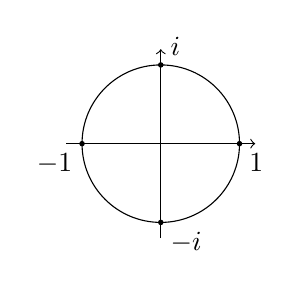
\begin{tikzpicture}
      \draw (0,0) circle [radius=1];
      \draw[->] (-1.2,0) -- (1.2,0);
      \draw[->] (0,-1.2) -- (0,1.2);
      \fill (1,0) circle[radius=1pt] node[below right] {$1$};
      \fill (-1,0) circle[radius=1pt] node[below left] {$-1$};
      \fill (0,1) circle[radius=1pt] node[above right] {$i$};
      \fill (0,-1) circle[radius=1pt] node[below right] {$-i$};
    \end{tikzpicture}
\end{center}
$$
0 + 1i = i \in S^1: i^1 = i, i^2 = -1, i^3 = -i, i^4 = 1 \text{ red elementa } i \text{ je 4}
$$
\begin{align*}
    -i \in S^1: (-i)^1 &= -i, (-i)^2 = (-i) \cdot (-i) = -1 \\
    (-i)^3 &= (-i)^1 \cdot (-i)^2 = -i \cdot (-1) = i \\
    (-i)^4 &= (-i)^2 \cdot (-i)^2 = (-1) \cdot (-1) = 1 \text{ red elementa } -i \text{ je 4}
\end{align*} \\

\noindent
c) $A = \mathbb{Z}$














\end{document}
